\documentclass[a4paper]{article}
\usepackage{fancyhdr}
\usepackage{physics}
\usepackage{graphicx}
\usepackage{hyperref}

\usepackage{subcaption}
\usepackage{floatrow}
\usepackage{fancyhdr}
\usepackage{afterpage}

\fancyhf{}
\pagestyle{fancy}
\rhead{\textcolor{gray}{Mock Draft}}

\graphicspath{ {img/} }

\title{Meine Antwort zum erweiterten Wigner's Freund Gedankenexperiment - Zweiter Teil/Version}
\author{Jannis Naske}

\pagestyle{fancy}
\fancyhf{}
\rhead{Jannis Naske}


\begin{document}


\maketitle
\afterpage{\cfoot{\thepage}}
\section*{Einführung}
In diesem Dokument beschreibe ich einen Fehler im erweiterten Wigner's Freund Gedankenexperiment von Renner und Frauchiger. Der Fehler liegt weder in den Grundannahmen, \textbf{(Q)}, \textbf{(C)}, und \textbf{(S)}, noch in den einzelnen Statements der Agenten, sondern darin wie diese Statements kombiniert werden. Die verwendeten Notationen, die ich hier verwende, entsprechen denen von Wikipedia(Link in den Referenzen), und nicht dem ursprünglichen Artikel.

\section*{Der Fehler}
Wir betrachten das Gedankenexperiment zu der Zeit, nachdem $F_2$ sein Qubit mit dem Resultat $\ket{\uparrow}$ gemessen hat. Statement 2, welches $F_2$ gibt, lautet:
\begin{itemize}
	\item \textbf{Statement 2 von} $F_2$: ``Wenn ich $\ket{\uparrow}$ messe, dann hat $F_1$ $\ket{t}$ gemessen.''
\end{itemize}
Hier ist es sehr wichtig zu bemerken, dass wenn dies der Fall ist, $F_2$ $F_1$'s Qubit in der Standardbasis mitgemessen hat. Dies wäre nicht der Fall, wenn $F_2$ $\ket{\downarrow}$ gemessen hätte. $W_1$ führt nun seine Messung aus. Da er nur $F_1$'s Qubit, beziehungsweise dessen Labor, misst, ist es auch wichtig, dass die Qubits, beziehungsweise die Labore, von $F_1$ und $F_2$ voneinander isoliert sind, wie dies in einem Quantenregister von einem Quantencomputer der Fall wäre. Da $W_1$ $F_1$'s Qubit in einer Superposition misst, endet es schliesslich auch in einer Superposition. Hier tritt das Problem auf: Da $F_2$ den Ablauf kennt, weiss $F_2$ nun dass obwohl er vorhin $\ket{\uparrow}$ gemessen hat, das Qubit von $F_1$ sich wieder in einer Superposition befindet. Er kommt also selber zum Schluss, dass sein Statement nicht mehr zu dieser Zeit gilt! Wenn am Schluss vom Experiment die Statements in der umgekehrten Reihenfolge aufeinander angewendet werden, kann Statement 2 nicht mehr aus Statement 3 gefolgert werden. Im originalen Artikel wird am Schluss Statement 2 falsch interpretiert, nämlich als: ``Wenn ich $\ket{\uparrow}$ messe, dann wird ab dann, während des Experiments, $F_1$ und sein Labor im Zustand $\ket{t}$ sein.''

\begin{figure}[!htb]
\begin{floatrow}[1]\
\ffigbox{\caption*{Gültigkeit für die Statements}}%
{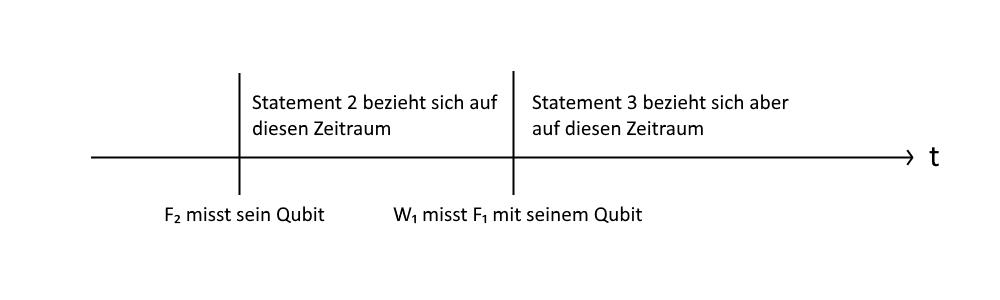
\includegraphics[width=1\textwidth]{neu.png}}
\end{floatrow}
\end{figure}

\pagebreak

\section*{Referenzen}
\begin{itemize}
	\item \url{https://en.wikipedia.org/wiki/Wigner%27s_friend}
	\item \url{https://www.ncbi.nlm.nih.gov/pmc/articles/PMC6143649/}
	\item \url{https://link.springer.com/book/10.1007/978-3-658-10455-9}
\end{itemize}


\end{document}